\documentclass[12pt,a4paper]{article}
\usepackage[utf8]{inputenc}
\usepackage[german]{babel}
\usepackage[T1]{fontenc}
\usepackage{amsmath}
\usepackage{amsfonts}
\usepackage{amssymb}
\usepackage{graphicx}
\usepackage[left=2.5cm,right=2.5cm,top=2cm,bottom=2cm]{geometry}
\author{Gruppe C14 \\ Julián Häck, Martin Koytek, Lars Wenning, Erik Zimmermann}
\usepackage{float}
\begin{document}
\section{Wärmelehre}
\subsection{Rauschen}
Rauschen auf p und T bei Zimmertemperatur im Glas.
Histogramm $\Rightarrow$ Fehler auf Einzelwert.
\begin{equation}
\sigma_p = \sqrt{\frac{\sum (p-\bar{p})^2}{n-1}}
\end{equation}
$\sigma_{\bar{p}}=\frac{\sigma_p}{\sqrt{n}}$

\begin{table}[H]\centering
\begin{tabular}{|c|c|}
\hline 
Intervall & 20ms \\ 
\hline 
Anzahl & 5000 \\ 
\hline 
Zeit & 100s \\ 
\hline 
\end{tabular} 
\end{table}
\subsection{Temperaturkalibration}
\begin{equation}
T_R=aT_C+b
\end{equation}
Eiswasser: $T_0^T=273.16K$, Siedetemperatur $T_{100}^T=T_0^T+T(p)$ 
\subsection{Dichtigkeit}
Mit Pumpe Unterdruck erzeugen 400-300 hPa \\
p gegen t auftragen \\
maximal $3\frac{hPa}{min}$ \\
\subsection{Hauptmessung}
Clausius Clapeyron: 
\begin{equation}
\frac{dp}{dT}=\frac{\nu \Lambda}{T(V_1-V_2)}
\end{equation}
Näherungen: $V_{Gas} >> V_{Fluessig}$, $pV=\nu RT$,\\
$\Rightarrow$
\begin{equation}
ln(p)=-\frac{\Lambda}{R}\frac{1}{T}+c
\end{equation}
erhitzen bis sieden, erst beim Abkühlen Messung starten. 
\begin{table}[H]\centering
\begin{tabular}{|c|c|}
\hline 
Intervall & 100ms \\ 
\hline 
Anzahl & $\infty$ \\ 
\hline 
Zeit & $\infty$ \\ 
\hline 
\end{tabular} 
\end{table}
\newpage
\section{Elektrotechnik}
\subsection{Gedämpfter LC Schwingkreis Oszilloskop + Cassy}
\begin{equation}
U_{n+1}=U_n e^{\delta(t_{n+1}-t_n)} \Rightarrow \delta_n=\frac{ln(\frac{U_n}{U_{n+1}})}{t_{n+1}-t_n}
\end{equation}
\begin{table}[H]\centering
\begin{tabular}{|c|c|}
\hline 
Intervall & 10 $\mu$ s \\ 
\hline 
Anzahl & 4000 \\ 
\hline 
Zeit & 40ms \\ 
\hline 
\end{tabular} 
\end{table}

\begin{figure}[H]
\centering
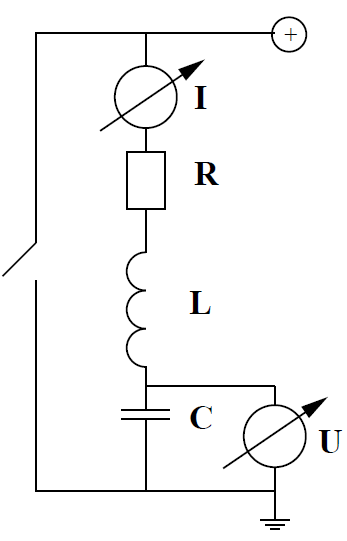
\includegraphics[scale=0.5]{GedLCSchwingkreis.PNG}
\caption{Gedämpfter LC Schwingkreis}
\end{figure}

Bei Oszillospkop auf Single Sequence stellen.\\
Offset vor dem logarithmieren abziehen.\\
$C=10\mu F, L=36mH, R_i=9.5 \Omega, R=0-220 \Omega$ Drehwiderstand
\subsection{Bestimmung der Induktivität}
\begin{equation}
\delta=\frac{1}{2L}\cdot R
\end{equation}
$\delta$ bei unterschiedlichen R messen.
\subsection{Schwingfälle}
\begin{equation}
\omega_0=\sqrt{\frac{1}{LC}}, \hspace{1cm} \omega=\sqrt{\omega_0^2-\delta^2}
\end{equation}
Aperiodischer Grenzfall
\begin{equation}
\omega_0=\delta \Rightarrow R_{ap}=2\sqrt{\frac{L}{C}}\stackrel{hier}{\approx}120\Omega
\end{equation}
Für den Kriechfall $R=1000 \Omega$
\end{document}